\documentclass[compress,11pt]{beamer}
%\includeonly{pendel}
\usetheme{Ilmenau}
%\usetheme{fau-4-3}
%\usecolortheme{beaver}
%\beamertemplatenavigationsymbolsempty
\usepackage[ngerman]{babel}
\usepackage{marvosym}
\usepackage{multimedia}
\usepackage[utf8x]{inputenc}
\usepackage{amsmath}
\usepackage{amsfonts}
\usepackage{amssymb}
\usepackage{graphicx}
\usepackage{esvect}
%\author{}
\title{EP Gruppe 8}
%\setbeamercovered{transparent}
%\setbeamertemplate{navigation symbols}{}
%\logo{}
%\institute{}
%\date{}
%\subject{}
\usepackage{verbatim}
\begin{document}
\section{Sequentielle Logik}
\subsection{RS-Flip-Flop}
\begin{frame}
\begin{block}{Schaltung}
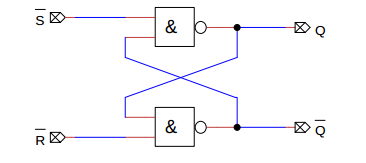
\includegraphics[scale=0.7]{rs}
\end{block}
\end{frame}
\begin{frame}
\begin{block}{Aufbau und Funktion}
\begin{itemize}
\item Zusammengesetzt aus zwei gekoppelten NAND-Gattern
\item Ausgänge sind (vom Zustand $\overline{S} = 0$ und $\overline{R} = 0$ abgesehen) invertiert
\item Durch Setzen von $\overline{S} = 1$ bzw.$\overline{R} = 1$ können die Ausgänge gesetzt weden
\item Wahrheitstafel des NAND-Gatters bewirkt, dass durch das Setzen der beiden Eingänge auf 1 der letzte Zustand des Flip-Flops ausgegeben wird - Flip-Flop kann Zustände speichern
\end{itemize}
\end{block}
\end{frame}
\begin{frame}
Wahrheitstafel:\\
\begin{tabular}{|c|c||c|c|}
\hline 
$\overline{S}$ & $\overline{R}$ & $Q$ & $\overline{Q}$ \\ 
\hline 
0 & 0 & (1) & (1) \\ 

0 & 1 & 1 & 0 \\ 
 
1 & 0 & 0 & 1 \\ 
 
1 & 1 & $Q_{n-1}$ & $\overline{Q_{n-1}}$ \\ 
\hline 
\end{tabular} 




\end{frame}
\subsection{Taktgesteuerter RS}
\begin{frame}

\begin{block}{Schaltung}
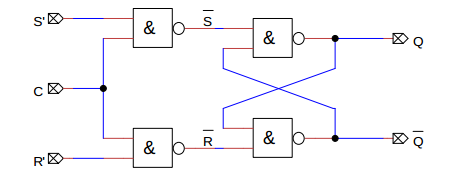
\includegraphics[scale=0.7]{taktrs}
\end{block}

\end{frame}
\begin{frame}
\begin{block}{Funktionsweise}
\begin{itemize}
\item Dem RS-Flip:Flop werden nun noch zwei NAND-Gatter vorrangestellt, die über das Clock-Signal verbunden sind
\item Solange $C = 0$ $\Rightarrow$ fester Anfangszustand, der nicht durch S und R beeinflusst wird, da NAND-Gatter $1$ ausgibt, sobald eines der Signale $0$ ist
\item Schaltung ist "flankengesteuert", also gesetzte $S$ und $R$ werden erst übernommen, wenn $C$ eingeschaltet wird
\end{itemize}
\end{block}
\end{frame}
\begin{frame}
\begin{block}{Verlauf der Schaltvorgänge}
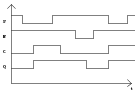
\includegraphics[scale=1.3]{trs}
\end{block}

\end{frame}
\subsection{D-Latch}

\begin{frame}
\begin{block}{Schaltung}
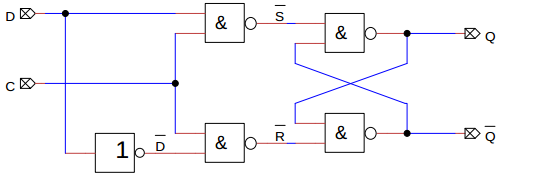
\includegraphics[scale=1]{dlatch1}

\end{block}

\end{frame}
\begin{frame}\begin{tabular}{|c|c||c|}
\hline 
$\overline{D}$ & $C$ & $\overline{S}$ \\ 
\hline 
1 & 0 & 1 \\ 

1 & 1 & 1 \\ 

0 & 0 & 1 \\ 

0 & 1 & 0 \\ 
\hline
\end{tabular} \\
Bis auf den irrelevanten Fall $C = 0$ (es findet keine Veränderung des Zustandes statt) sind $\overline{D}$ und $\overline{S}$ identisch
\end{frame}
\begin{frame}
\begin{block}{Schaltung kann somit vereinfacht werden}
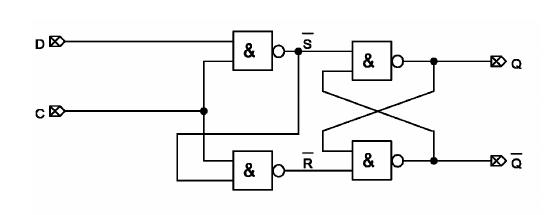
\includegraphics[scale=0.7]{dlatcheinfach}
\end{block}
\end{frame}
\begin{frame}
\begin{block}{Funktionsweise}
\begin{itemize}
\item $R$ zu $S$ negiert, daher existiert kein unbestimmter Zustand
\item Schaltung nicht flanken- sondern zustandsgesteuert: sobald $C = 1$, lassen sich Zustände setzen bzw. überschreiben
\end{itemize}
\end{block}
\end{frame}
\begin{frame}
\begin{block}{Verlauf der Schaltvorgänge}
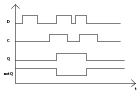
\includegraphics[scale=1.3]{dlatch}
\end{block}
\end{frame}
\begin{frame}
\begin{block}{Wahrheitstafel}
\begin{tabular}{|c|c|c|}
\hline 
$D$ & $C$ & $Q$ \\ 
\hline 
x & 0 & $Q_{n-1}$ \\ 
\hline 
0 & 1 & 0 \\ 
\hline 
1 & 1 & 1 \\ 
\hline 
\end{tabular} 

\end{block}
\end{frame}
\subsection{Flankengesteuertes RS-Flip-Flop}
\begin{frame}
\begin{block}{Schaltung}
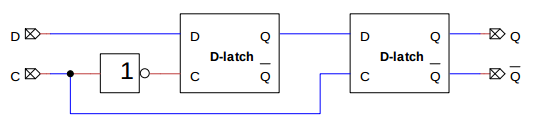
\includegraphics[scale=0.7]{flanke}
\end{block}
\end{frame}
\begin{frame}
\begin{block}{Funktionsweise}
\begin{itemize}
\item Bei $C$ konstant wird der zuletzt gesetzte Wert von $Q$ rückgegeben
\item Sobald steigende Flanke auf $C$, wird $Q$ = $D$ gesetzt
\end{itemize}
\end{block}
\end{frame}
\begin{frame}
\begin{block}{Verlauf der Schaltvorgänge}
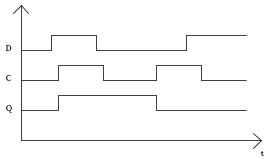
\includegraphics[scale=1]{triggerrs}
\end{block}
\end{frame}
\begin{frame}
\begin{block}{Wahrheitstafel}
\begin{tabular}{|c|c|c|}
\hline 
$D$ & $C$ & $Q$ \\ 
\hline 
x & 0 & $Q_{n-1}$ \\ 

n & Steigende Flanke & n \\ 
 
x & 1 & $Q_{n-1}$ \\ 
\hline 
\end{tabular} 
\end{block}
\end{frame}


\section{Zähler}
\begin{frame}
\begin{block}{Schaltung}
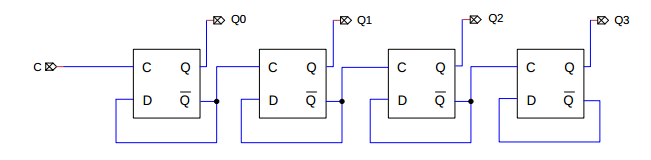
\includegraphics[scale=0.6]{zahler}
\end{block}
Es kann so Addition der Flankensignale in Binärform realisiert werden
\end{frame}
\begin{frame}

Durchführung mit 2 * 2 flankengetriggerten D-Flip-Flops in IC-Form

\begin{block}{Funktionsweise}
\begin{itemize}
\item $D$ immer mit $Q$ verbunden, also wechselt $Q$ bei jeder Flanke den Wert
\item Da Flip-Flop flankengetriggert, nur Reaktion auf einfaches Betätigen des Schalters
\item Bei Setzen von $Q$ auf 0 wird $\overline{Q}$ auf 1 gesetzt und die anderen Bits erhalten ein Schaltsignal
\end{itemize}
\end{block}
\end{frame}
\begin{frame}
\begin{block}{Eigenschaften}
\begin{itemize}
\item Speicher = 4 Bit, somit ist maximale darstellbare Zahl 15
\item Wenn Wert des Zählers gleich 15, sind alle $Q$ = 1, bei einer weiteren Flanke werden alle $Q$ wieder auf 0 gesetztc $\Rightarrow$ kein Übertrag möglich
\end{itemize}
\end{block}
\end{frame}

\section{binary coded decimal und 7-­Segment­-Anzeige}
\subsection{BCD}
\begin{frame}
Ziel: Darstellung der Binärzahl des Zählers als gewohnte Dezimalzahl, Realisierung über speziellen IC sowie kompatibler Anzeige
\begin{block}{Schaltung}
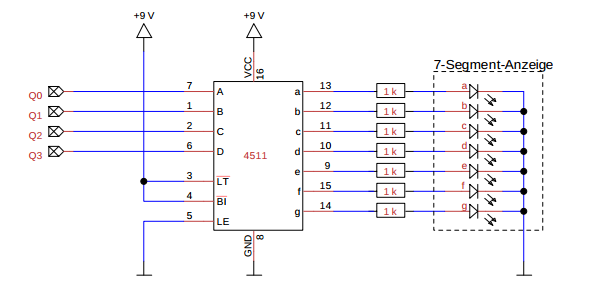
\includegraphics[scale=0.7]{a5sch}

\end{block}
\end{frame}
\begin{frame}
\begin{block}{Wahrheitstafel des CMOS 4511}
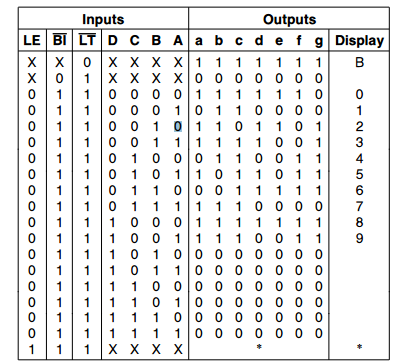
\includegraphics[scale=0.7]{a5tafel}

\end{block}
\end{frame}
\begin{frame}
\begin{block}{Funktionsweise}
\begin{itemize}

\item CMOS 4511 wandelt Binärzahl in BCD-Code, um mit 7-Segment-Anzeige kommunizieren zu können, die die Zahl in Dezimal-Darstellung anzeigen kann
\item CMOS nur für Verwendung mit einstelliger Anzeige konstruiert/geeignet, denn sobald $(1001)_2 = 9_{10}$, also die größte einsstellige Dezimalzahl überschritten wird, gibt Chip nur noch Signale $a \dots f = 0$ zurück $\Rightarrow$ keine Anzeige
\end{itemize}
\end{block}
\end{frame}
\subsection{Würfel}
\begin{frame}
Mit Frequenzgenerator, der Rechtecksspannung ausgibt, kann nun das Zählen automatisiert werden, also es werden alle einkommenden Flanken gezählt, wobei sich der Zähler nach 15 Signalen wieder zurücksetzt\\
Dies lässt sich auch nutzen, um bei hohen Signalfrequenzen mit der Schaltung Zufallszahlen zu erzeugen.\\
Dem Zähler aus Aufgabe 4, der über die $Q_i$ mit der Schaltung aus Aufgabe 5 verbubńden ist, wird noch ein Schalter vorrangestellt.\\
Sobald dieser gedrückt, erreichen Pulse die Schaltung, und da die Anzahl dieser bei hohen Frequenzen nicht mehr abgeschätzt werden können, ist die Anzeige zufällig.
\end{frame}
\begin{frame}
Problem: Noch zählt der Zähler nicht dezimal, sondern bis 15 wobei bei 11 bis 15 die Anzeige inaktiv ist 
\begin{block}{Behebung}
\begin{itemize}
\item Zähler muss beim erreichen der Zahl $(10)_{10}$ = $(1001)_2$ wieder auf den Wert 0 gesetzt werden
\item Wird realisiert, indem die Pegel $A$ und $D$ mit AND-Gatter auf die Reset-Pins der mit $A$ und $D$ verbundenen Flip-Flops verbunden werden 
\end{itemize}
\end{block}
Nun funktioniert Schaltung wie erwartet
\end{frame}
\end{document}
